%!TEX root = D2.1_AMIDSTModellingFramework.tex

\newpage
\newpage
\newcommand{\X}{\mathbf{X}}
\newcommand{\Y}{\mathbf{Y}}
\newcommand{\Z}{\mathbf{Z}}

\subsection{CajaMar Models}
\label{Section:CajaMarModels}

\subsubsection{Introduction}

There are two tasks to be solved for Cajamar's use case (see D1.2 and DoW). The main one is
the estimation of the \emph{probability of default}, defined as the probability that a
credit operation will end up in default within two years. The secondary task consists in obtaining 
good customer profiles in terms of risk, so that marketing campaigns can be
specifically targeted to these low risk customers. 

%%%%%%%%%%%%%%%%%%%%%%%%%%%%%%%%%%%%
\subsubsection{Predicting probability of default}
\label{SubSection:Predicting}
%%%%%%%%%%%%%%%%%%%%%%%%%%%%%%%%%%%%

%---------------------------------------------------------------------------------------------
\subsubsection*{Introduction of the problem} 

In any commercial bank, every time a customer applies for a loan, the bank experts evaluate the customer's risk profile before making their decision. 

At Cajamar, this risk evaluation protocol is implemented by evaluating whether the client is going to default or not within the following two years. When a client is labelled as defaulter, he/she will remain defaulter in the database at least two more years, so the client will become non-defaulter again when everything has been paid appropriately during the last 2 years. 

The problem of predicting the customer risk of default is currently addressed at Cajamar by an automatic supervised classification model (i.e. a logistic regression). It takes information about the recent financial activity of a customer, as well as information about recent past paying behaviour provided by other Spanish financial institutions. Finally, using this information, predictions about the probability that the client will default during the following two years are made. The methodology currently employed does not assume dependence structure among the variables and current predictions are made using only a set of $27$ variables out of more than $1000$ available. Updates in risk predictions are made on a monthly basis, whereas the predictive model is only updated after several years. These low update frequencies are partly due to limitations in the available commercial software and the computing resources.

The objective is to daily update the risk of default for every customer of the bank. This daily evaluation will be made by creating two data sets: the model training data set and the model evaluation data set (see Use Case 1 in D1.2). How these data sets are created gives us some insights about the nature of this risk prediction problem.  Figure~\ref{Figure:CajaMarTimeLine} show how the evaluation and training datasets are generated within a time-line. The current time is denoted as $t$ and the time $2$ years back as $k$, i.e., $k=t-2$ years. 

\begin{figure}[htbp]
\centering
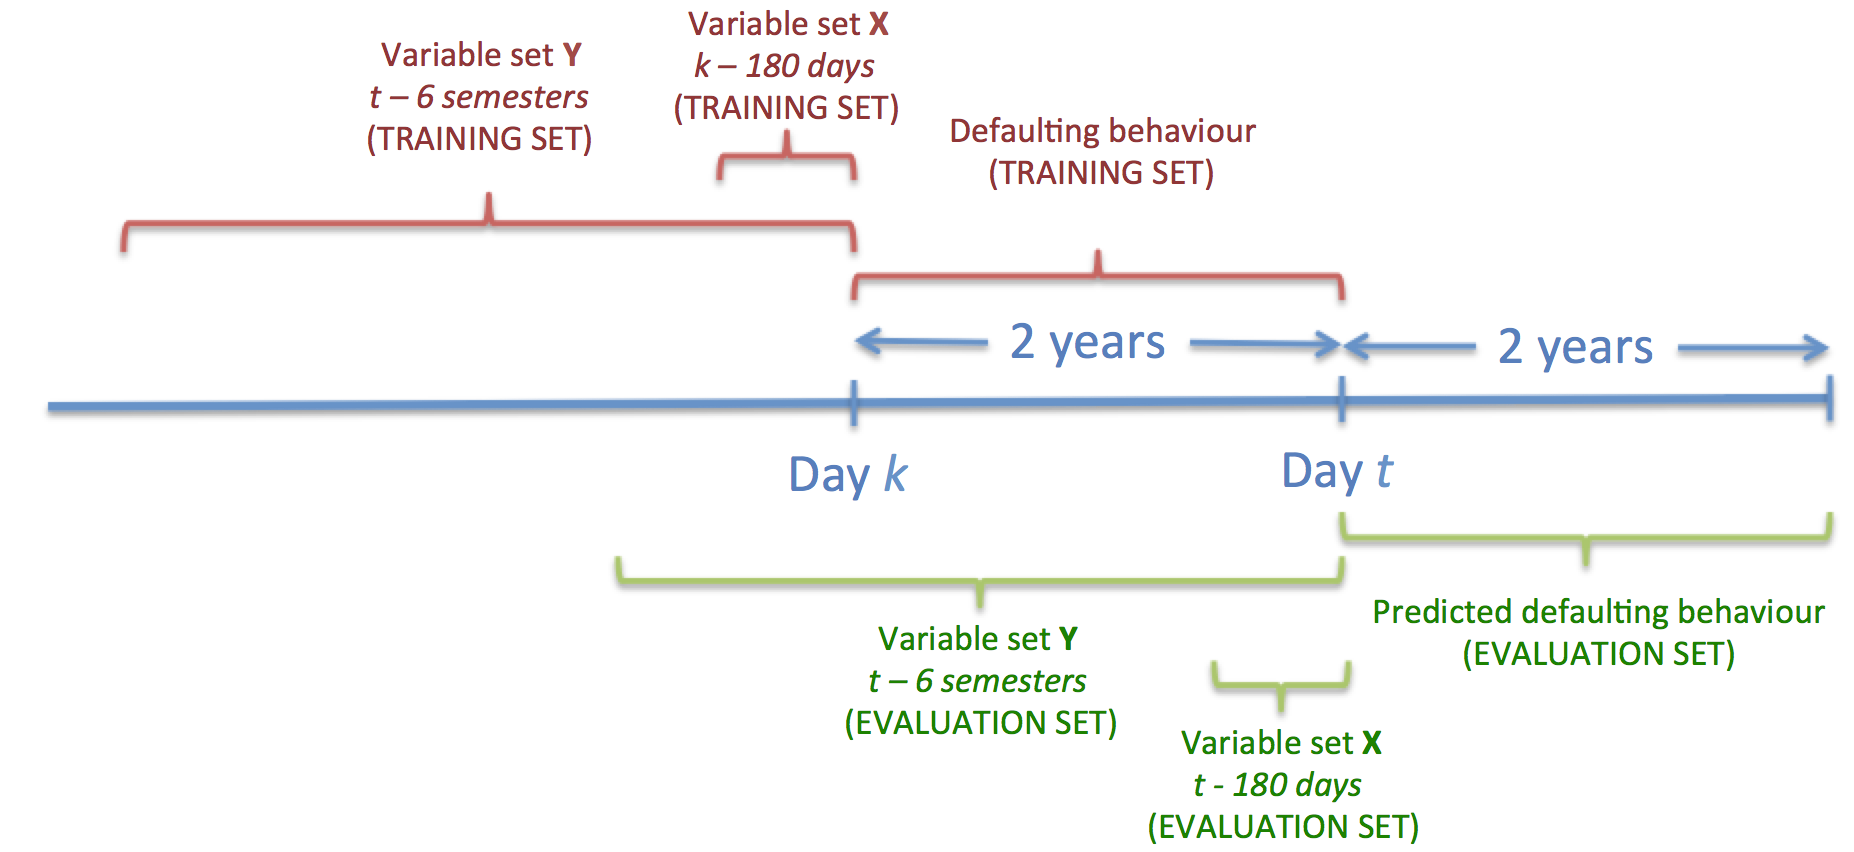
\includegraphics[scale=0.4]{figures/CajaMarTimeLine}
\caption{\label{Figure:CajaMarTimeLine}Time-line showing how the evaluation and training data sets are generated.}
\end{figure}

\begin{itemize}
\item \textbf{Model Evaluation Data Set:} The evaluation data set is created at time $t$. This data set contains a record for every client to be evaluated. Note that, data about the predicted defaulting behavior is still missing at time $t$ when conforming the evaluation dataset. It will be obtained after performing inference on the model. As in any standard evaluation data set in supervised classification settings, each record will contain the values of the predictors variables for this customer. The predicting variables refers to the financial activity and the paying behaviour of the customers in a recent past, and their socio-demographic data. 

The recent {\bf financial activity} of a customer refers to attributes such as ``account balance'', ``number of credit card operations'', etc. in the last 180 days\footnote{This limit is fixed by the Bank of Spain}. These attributes usually change daily for a customer, so they are encoded by introducing a set of variables for each attribute, one for each day back from current time $t$. Hence, the financial activity of a customer is specified by a number of variables equals to 180 times the number of predictors. 

In the case of {\bf past paying behaviour}, the attributes refers to variables such as payments inside Cajamar (loans, mortgages, credits, etc.). A record of the last 36 months divided by semester is considered when building the evaluation data set. So, a number of variables equals to $6$ times the number of attributes referring to the paying behaviour are used in this case. Moreover, some other static variables with information about payments to other financial institutions or companies (phone and electricity bill, public bodies, etc.) is included in this group of variables.

The dataset for the evaluation of customers is detailed in Table~\ref{tab:EvaluationDataset}. Note that there exist another group of variables denoted as $\Z$ (mainly sociodemographic variables) that are not replicated over time as they remains fixed. 
%The data included in both data sets regarding these variables refer to time $t$.


\begin{table}[htbp]
\centering
\begin{tabular}{c|ccc|ccc|c}
	&\multicolumn{3}{c|}{Days} & \multicolumn{3}{c|}{Semester} \\
     Time $t$              & $\X^{(t-180)}$ & $\ldots$ & $\X^{(t-1)} $ & $\Y^{(t-6)}$  & $\ldots$ & $\Y^{(t-1)} $ & $\Z$  \\  
\hline
Client$_1$  &                                                  &              &                     &                               &                     &        \\ 
$\vdots$      &                                                 &               &                     &                                &                     &      \\ 
Client$_n$  &                                                &               &                     &                                &                     &     \\ 
\end{tabular}
\caption{Evaluation dataset at time $t$. Attributes for financial activity, paying behavior and sociodemographic information are denoted as $\X$, $\Y$ and $\Z$, respectively.}
\label{tab:EvaluationDataset} 
\end{table}

In conclusion, the idea is to take each of the records (i.e. customers) of this data set and compute the probability of defaulting within the following two years. Finally, the risk table in the system is updated (see Table~\ref{tab:riskTable}).

\begin{table}[h]
\centering
\begin{tabular}{c|ccc|ccc|c}
     Time $t$  & Risk of defaulting \\  
\hline
Client$_1$  &    $r_1$  \\ 
$\vdots$      &   $\vdots$   \\ 
Client$_n$  &   $r_n$  \\ 
\end{tabular} 
\caption{Table containing the risk of defaulting for every client.}
\label{tab:riskTable}
\end{table}


If at some point the probability of defaulting of some customers rises above some predefined threshold, the bank considers taking preventive actions to reduce the chances of defaulting by the customer.

\item \textbf{Model Training Data Set:}  The training data set is built in the same way as the evaluation data set. They contain the same set of predictive variables plus the \emph{Defaulter} variable. The main difference is they refer to different time points. The predictive variables in the evaluation data set are built from time $t$ (current time) backward, whereas the ones in the training data set are built from time $k$ (2 years before $t$) backward. The dataset for training/updating the model is detailed in Table~\ref{tab:TrainingDataset}.
\begin{table}[h]
\centering
\begin{tabular}{c|ccc|ccc|c|c}
	&\multicolumn{3}{c|}{Days} & \multicolumn{3}{c|}{Semester} & \\
     Time $t$              & $\X^{(k-180)}$ & $\ldots$ & $\X^{(k-1)} $ & $\Y^{(k-6)}$  & $\ldots$ & $\Y^{(k-1)} $ & $\Z$ & Defaulter$^{(t)}$\\  
\hline
Client$_1$  &                                                  &              &                     &                               &                     &        &  \\ 
$\vdots$      &                                                 &               &                     &                                &                     &       & \\ 
Client$_n$  &                                                &               &                     &                                &                     &     & \\ 
\end{tabular} 
\caption{Training dataset at time $t$ with $k=t - 2$ years.  The notation is the same as in Table~\ref{tab:EvaluationDataset}.}
\label{tab:TrainingDataset} 
\end{table}

Unlike the evaluation data set, each record contains a class label indicating if this customer is defaulter o non-defaulter as predicting variables data are prepared in such a way that information about defaulting behavior is available at time $t$. To decide if a customer is defaulter or not, we look at the data 2 years back from current time $t$. If during these two years there are not any evidence of defaulting and the client's payments (at Cajamar and other financial institutions) has gone as expected, the client is labelled as non-defaulter. Otherwise, it is labelled as defaulter.

\end{itemize}

Next, we propose two modeling solutions for the risk prediction problem.



\subsubsection*{Static Model} 

In this first approach we do not explicitly consider some of the dynamics of the problem: we do not model that a customer can be non-defaulter and defaulter at different moments in time (e.g. one customer can be creditworthy and, after some time, go bankrupt due to unemployment). Instead, we consider a static prediction model where given the financial behaviour of the client over a recent past, it predicts whether the client will default or not within the next 2 years. Similarly to what it is done in the current Cajamar approach. 

Figure \ref{Figure:CajaMarStatic} shows the general structure of this static model. The payment variables are grouped by semesters whilst the financial activity variables by day. Note that past sociodemographic information are not necessary as it does not change frequently.
%For the sake of simplicity, for now on and in the graphical models depicted, we do not explicitly show the variables that refer to monthly information during the last 36 months. 

\begin{figure}[htbp]
  \centering
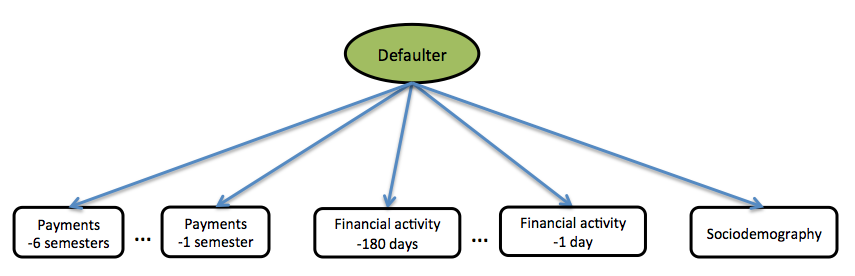
\includegraphics[scale=0.5]{./figures/CajaMarModel0}
\caption{\label{Figure:CajaMarStatic}Global structure of the static model. Each white box represents a set of variables for a particular time. The green node on top is the class variable \emph{Defaulter} that represents the probability that a customer will default within the next two years. } 
\label{fig:CajamarStaticModel}
\end{figure}

Expert knowledge from the bank point out that predicting variables are expected to be related so they might be connected within each box (e.g. according to a tree structure and, globally, conforming a TAN). 




%Figure~\ref{fig:CajaMarBayesianNetwork} shows a Bayesian network structure learnt from customers data that have been aggregated from different times, e.g., 180 times for financial activities \textcolor{red}{(We think it has no influence to get more dependences in the network structure)}
%To computationally simplify this learning in this preliminary overview,  \textcolor{blue}{only data correspond to one day?} are considered, meaning that the number of cases for learning has been considerably reduced. 
%Looking at the structure is evident that indeed there exist dependences between some of the variables\footnote{For confidentially reasons variable names are not shown}. The structure has been learnt using the R package \texttt{bnlearn}~\cite{Scu10, Nag13}.
%
%\begin{figure}[htbp]
%  \centering
%    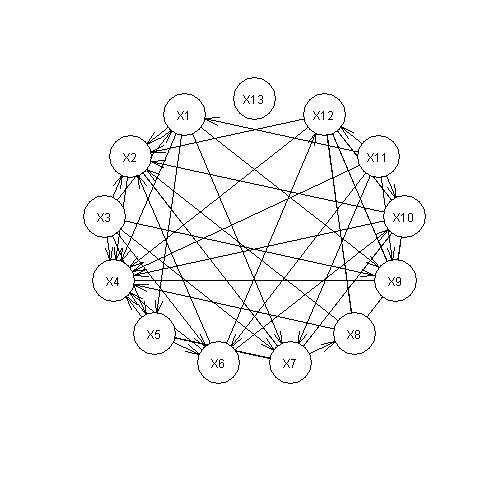
\includegraphics[width=70mm]{figures/CajaMarBayesianNetwork}
%    \vspace{-1cm}
%    \caption{Bayesian network structure learnt from 13 variables randomly chosen from the whole set of variables.}
%    \label{fig:CajaMarBayesianNetwork}
%\end{figure}


%
%
%\begin{figure}[htbp]
%  \centering
%    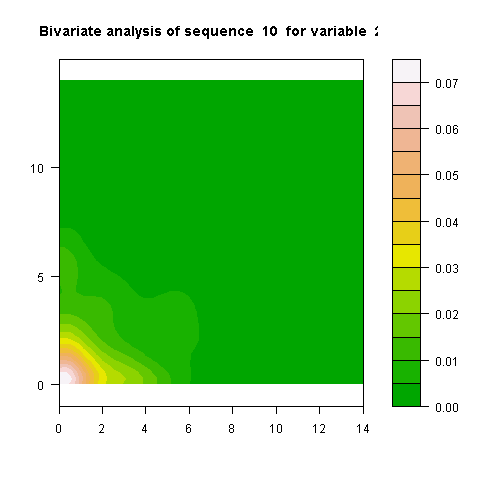
\includegraphics[width=70mm]{figures/CajaMarbv4}
%    \caption{Contour plot with (ideally) strong linear correlation between two variables \textcolor{blue}{(maybe class-conditioned?).}}
%    \label{fig:CajamarContourPlot}
%\end{figure}



%Figure \ref{fig:CajamarContourPlot} shows the contour bivariate plot for two variables, showing a clear linear relationship between them. 
Moreover, it may happen that one variable is even a replica of the other or contain quite similar information
%This might even indicate that one variable is just a replica of the other or contain quite similar information, 
and their joint contribution will not only make learning and inference computationally more expensive, but it could lead to poorer performance. This would contribute to support the need to explore suitable feature selection techniques as specified in Use Case 2 of Cajamar's Requirement analysis\cite{Fer14b}.

It is also of major interest to analyse the type of density probability distributions to use in the proposed model. Figures \ref{Figure:cajamarMixt} shows the density histogram for the values of one continuos attribute for defaulters and non-defaulters respectively. The density curves represent a credible approximation using mixture of Gaussian distributions, which is the case for most of the other predictive attributes. Note that for defaulters, the values of the \emph{end-of-day balance} are overall lower compared to those corresponding to non-defaulters.

\begin{figure}[htbp]
  \centering
    \begin{tabular}{cc}
    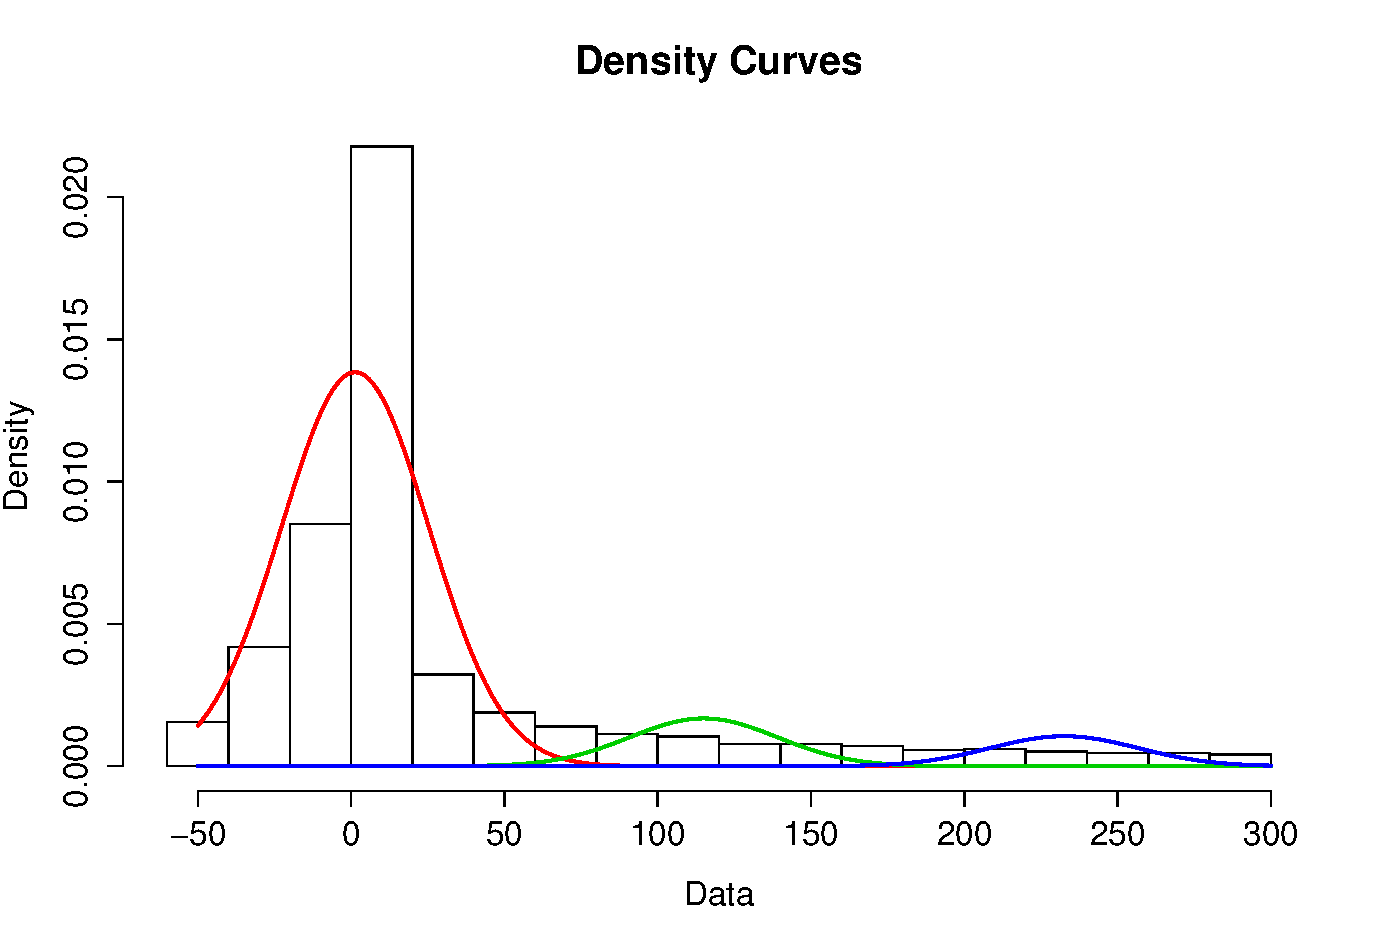
\includegraphics[width=70mm]{figures/CajaMarmixtureBalanceDef}&
    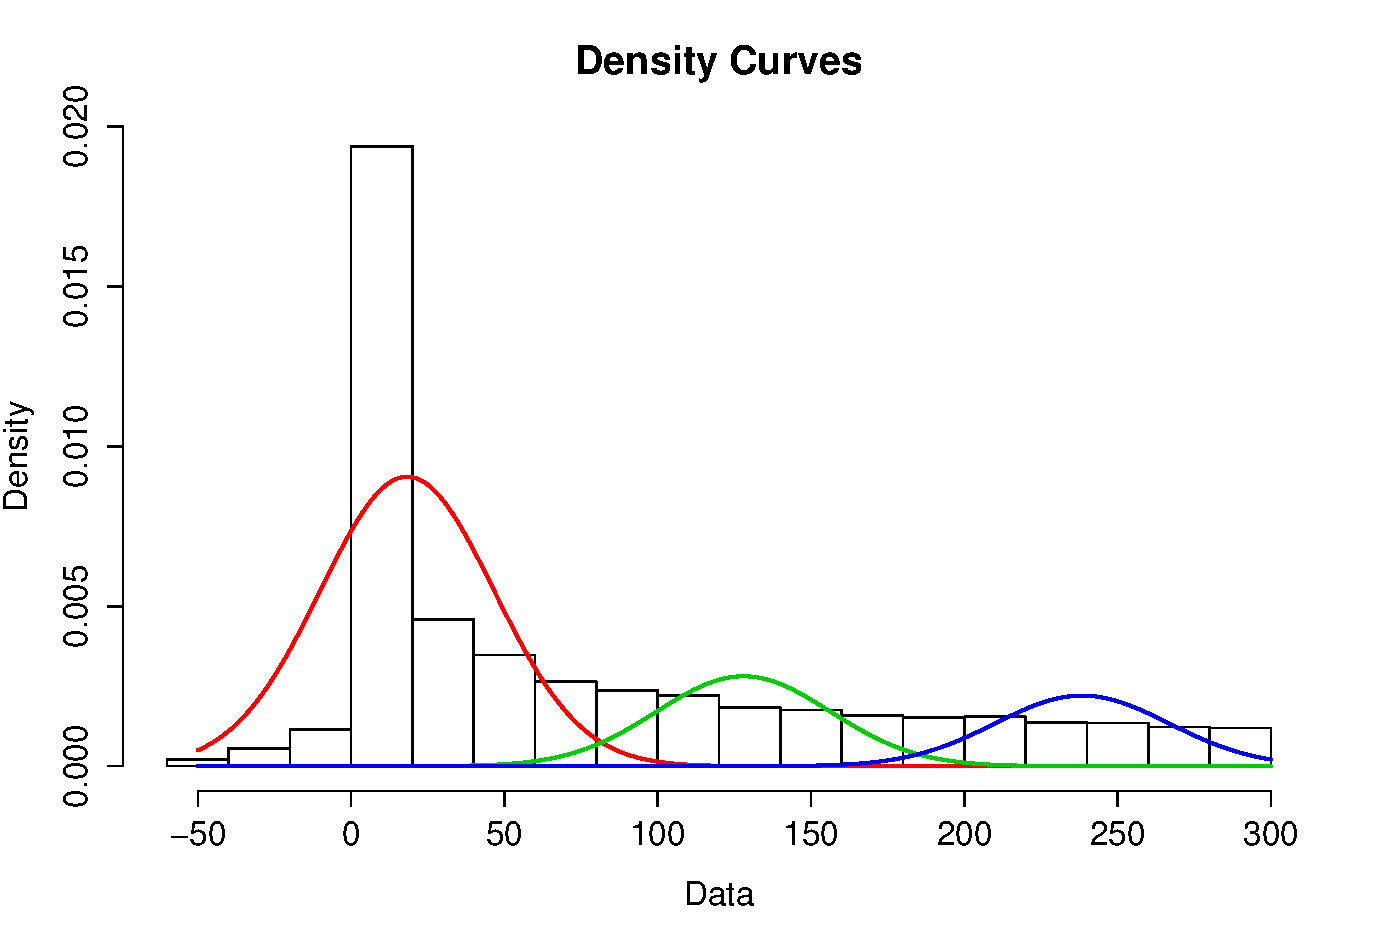
\includegraphics[width=70mm]{figures/CajaMarmixtureBalanceNonDef}\\
  \end{tabular}
    \caption{\label{Figure:cajamarMixt}Mixture of Gaussian approximation of one predicting variables conditioned to defaulter (left) and non-defaulter (right) value of the class variable.}
\end{figure}

There exist however discrete (non-ordinal) predictive attributes which impose a limitation in the structure of the Conditional Gaussian network, since discrete attributes cannot have continuous parents as pointed out in Section~\ref{SubSection:HybridBNs}. This might not be a problem for the semi-naive Bayesian network to be considered, and it is certainly not a problem for naive Bayes. Nonetheless, if this limitation were found to be problematic, then other probability distributions families will be explored, such as Mixture of Truncated Basis Functions~\cite{Lan12}, which can cope with any generic model structure. 

In summary, the process of building this static model consists of the following steps:

\begin{enumerate}
\item Using a set of SQL queries over the main relational dataset, a single flat table containing the information for training the model (see Table~\ref{tab:TrainingDataset}) is constructed every day. Note that, for instance, for variables related to financial activities, training data between two consecutive days $t$ and $t+1$ only differ in the new data arriving at day $t+1$ and obviating the data from 180 days ago at day $t$. Similar idea is applied for the paying behaviour variables.
\item Update the existing Bayesian network classifier with the new data.  Although relationships are more common between variables within each box, dependences among variables in different boxes are also allowed. 
\item Construct a single flat table with latest information about customers (evaluation dataset) in order to compute the latest risk profiles. This dataset was depicted in Table~\ref{tab:EvaluationDataset}.
\item Update the risk in Table~\ref{tab:riskTable} for every customer by propagating each record from the evaluation dataset in the static classifier obtained in Step 2. 
\end{enumerate}


%\begin{figure}[ht]
%\begin{center}
%\begin{tikzpicture}[->,>=stealth,shorten >=1pt,auto,node distance=2cm,semithick,
%        amarillo/.style={fill=yellow,rectangle,draw},
%        rojo/.style={fill=red,rectangle,draw,rounded corners}]
%        \node[green] (default) {Default};
%        \node (dot) [below of=default] {$\cdots$};
%        \node[amarillo] (tran1) [left of=dot] {Day -180};
%        \node[amarillo] (tran180) [right of=dot] {Day -1};
%        \draw (default) to (tran1);
%        \draw (default) to (tran180);
%\end{tikzpicture}
%\end{center}
%\caption{\label{Figure:CajaMarStatic}Global structure of the static model. Each yellow box represents a set of variables measures during the same day.
%The variables within a box can be connected (according to a tree structure and, globally, conforming a TAN).}
%\label{fig:static}
%\end{figure}
%---------------------------------------------------------------------------------------------



%\begin{figure}[ht]
%\begin{center}
%\begin{tikzpicture}[->,>=stealth,shorten >=1pt,auto,node distance=3cm,semithick,
%        amarillo/.style={fill=yellow,rectangle,draw},
%        rojo/.style={fill=red,rectangle,draw,rounded corners}]
%        \node[rojo] (default1) {Default -180};
%        \node[amarillo] (tran1) [below of=default1] {Day -180};
%        \node[rojo] (default2) [right of=default1] {Default -179};
%        \node[amarillo] (tran2) [below of=default2] {Day -179};
%        \node (dot) [right of=tran2] {$\cdots$};
%        \node (blank) [above of=dot] {$~~$};
%        \node[amarillo] (tran180) [right of=dot] {Day -1};
%        \node[rojo] (default180) [above of=tran180] {Default -1};
%        \draw (default1) to (tran1);
%        \draw (default2) to (tran2);
%        \draw (default180) to (tran180);
%        \draw (default1) to [bend left=45] (default2);
%        \draw (default2) to [bend left=45] (blank);
%        \draw (blank) to [bend left=45] (default180);
%        \draw (tran1) to [bend right=45] (tran2);
%        \draw (tran2) to [bend right=45] (dot);
%        \draw (dot) to [bend right=45] (tran180);
%\end{tikzpicture}
%\end{center}
%\caption{Global structure of the dynamic model. Each yellow box represents a set of variables measures during the same day.
%The variables within a box can be connected (according to a tree structure and, globally, conforming a TAN) as well as variables between two consecutive days. Red box refer to the possibility that 
%client is defaulter and are temporal connected.}
%\label{fig:global_temp}
%\end{figure}
%---------------------------------------------------------------------------------------------


%---------------------------------------------------------------------------------------------
\subsubsection*{Dynamic Model} 

In this second approach, we will consider the dynamic structure of the problem because the behaviour of the customers evolves over time (e.g. the account balance is continuously changing from one month to another, also the incomes, ...)  as well as the label as a defaulter or non-defaulter customer (e.g. customers can be creditworthy and, after some time, go bankrupt because they have lost their job). 


%\textcolor{red}{Analysing some of the data, we can actually see that if a customer was a defaulter at day $t$, the probability of being a defaulter at day $t+1$ changes from $p$ (prior probability in the static model) to $p'$ (transition probability in the dynamic model). The reason for this dramatic change is that once a client is a defaulter, he/she will be a defaulter for some time, and the static model is unable to represent this effect. }\textcolor{red}{ And the way we have defined the problem it actually does not matter much, does it? ANTONIO: I DON'T REALLY UNDERSTAND THIS PARAGRAPH} 




%\begin{figure}[ht]
%\begin{center}
%\begin{tikzpicture}
%  \node[circle,fill=yellow,draw, minimum size=1.1cm] (Xt1) at (1,1) {$X_{t-1}$};
%  \node[circle,fill=yellow,draw, minimum size=1.1cm] (Xt) at (5,1) {$X_t$};
%  \node[circle,fill=green,draw, minimum size=1.1cm] (avg) at (3,3) {$\bar{X}_t$};
%  \node[circle,fill=cyan,draw, minimum size=1.1cm] (ind) at (3,-2) {$\delta_{X_t}$};
%  \node[circle,fill=red,draw, minimum size=1.1cm] (D) at (5,5) {$D_t$};
%  \node[circle,fill=red,draw, minimum size=1.1cm] (Dt1) at (1,5) {$D_{t-1}$};
%  
%  \node at (0,3) {$\cdots$};
%  \node at (6,3) {$\cdots$};
%  
%  \draw[->] (Dt1) to (Xt1);
%  \draw[->] (Dt1) to (D);
%  \draw[->] (D) to (Xt);
%  \draw[->] (D) to (avg);
%  \draw[->] (Xt1) to (Xt);
%  \draw[->] (avg) to (Xt);
%  \draw[->] (ind) to (Xt);
%  
%  
%  
%\end{tikzpicture}
%\end{center}
%\caption{Basic component of the structure of the dynamic model.}
%\label{fig:component}
%\end{figure}




Figure~\ref{fig:global_temp} represents the global idea of the proposed temporal model. It can be compactly represented by a dynamic Bayesian network made of components as the one displayed in 
Figure~\ref{fig:component}. $D_t$ represents the class variable at time slice $t$ (i.e. defaulting or non-defaulting client). Each feature variable at time $t$, denoted as $X_t$, is linked to the same variable at time $t+1$, $X_{t+1}$. Although this is a reasonable assumption for most of the variables, this first Markov order relationship however might prove insufficient for some of the variables.

$\bar{X}_{t-1}$ and $\bar{X}_{t}$ represents memory variables at time $t$ and $t+1$ respectively. The inclusion of these type of variable might be necessary when we have evidence that first order Markov relationships does not hold and we need to account for information coming from the past. This evidence could be obtained from a partial correlogram as mentioned in Section~\ref{SubSubSection:StructuralAsumptions}.

Figure~\ref{fig:CajamarPartialCorrelograms} show a correlogram for a continuous predictive variable. The correlogram drop to almost zero for a lag equal to $2$, making a first Markov order assumption reasonable. However, a higher order could also rise from data, meaning that even earlier samples still could have an influence on the current sample given the previous one. 
%However, the right correlogram takes more time to drop to zero, which might indicate that 
To avoid building complex dynamic models with high Markov order, and to mitigate this effect,  a \emph{memory variable}, $\bar{X}_t$, has been included. For instance, a memory variable representing the average value during the last $180$ days could capture these dependences. Another reason to include these memory variables is that, even though they are computed from others, they provide information that might be disperse in the data and hardly can be captured with other variables as a whole. 

\begin{figure}[htbp]
\begin{center}
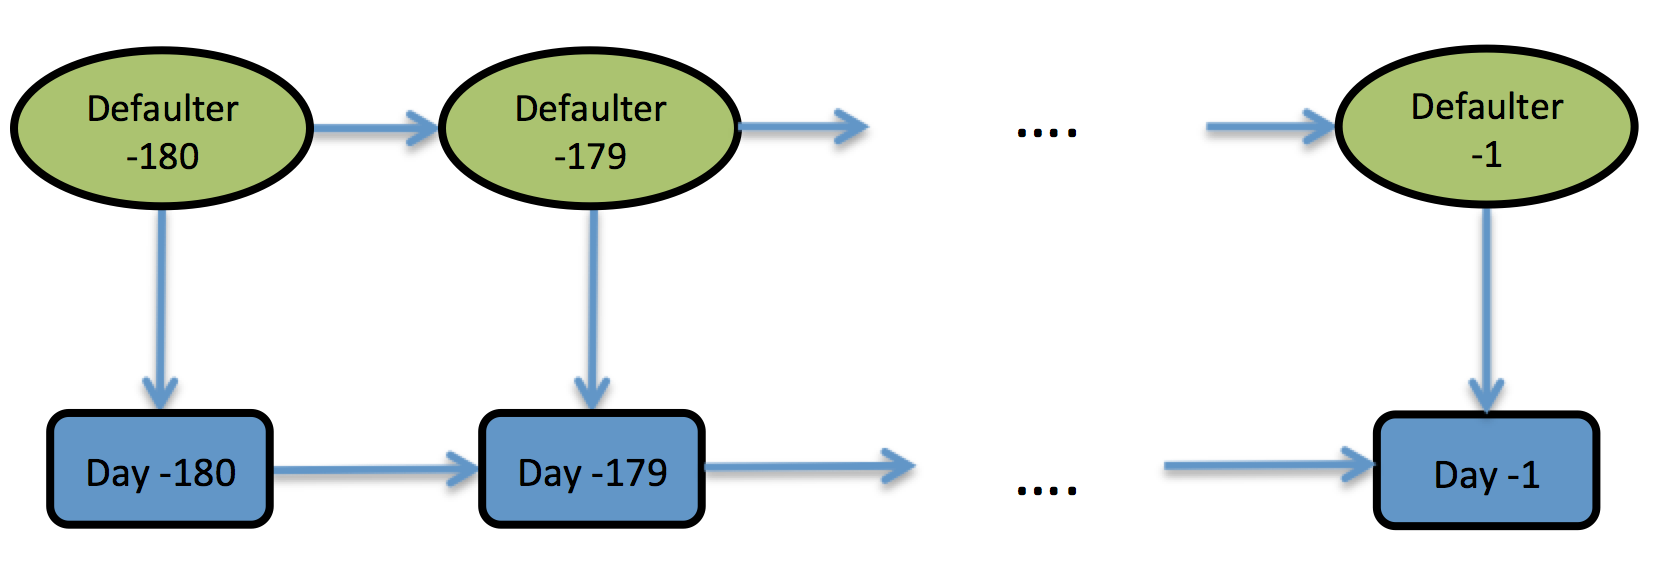
\includegraphics[scale=0.45]{./figures/CajaMarModel1}
\caption{Global structure of the dynamic model. Each white box represents a set of variables measures during the same day.
The variables within a box can be connected as well as variables between two consecutive days representing the same attribute. For the ease of presentation past paying behaviour and sociodemographic variables are omitted from now on.}
\label{fig:global_temp}
\end{center}
\end{figure}

\begin{figure}[htbp]
\begin{center}
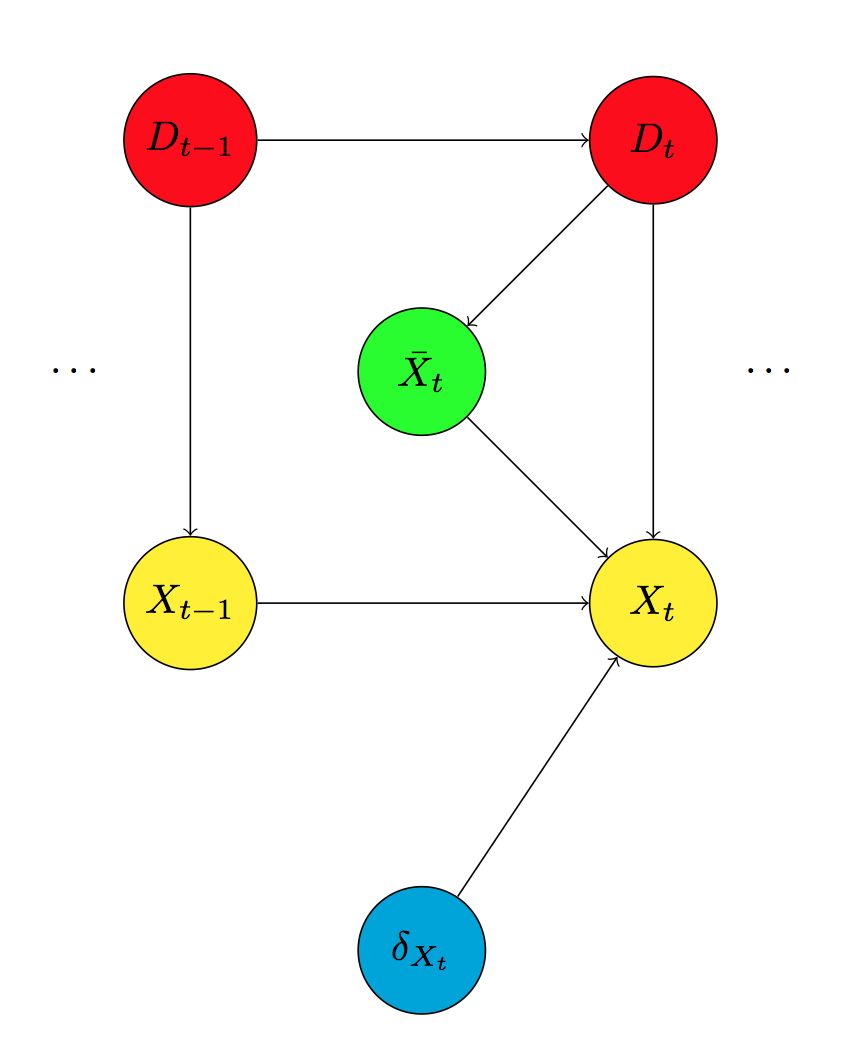
\includegraphics[scale=0.45]{./figures/CajaMarModel2}
\caption{Basic component of the structure of the dynamic model.}
\label{fig:component}
\end{center}
\end{figure}

\begin{figure}[htbp]
  \centering
   \begin{tabular}{cc}    
       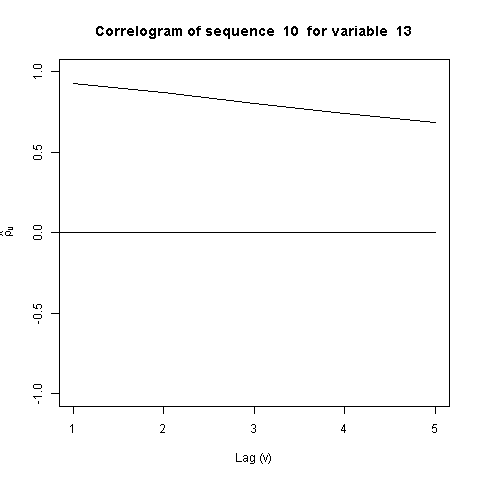
\includegraphics[width=70mm]{figures/CajamarCorrelogram} &
        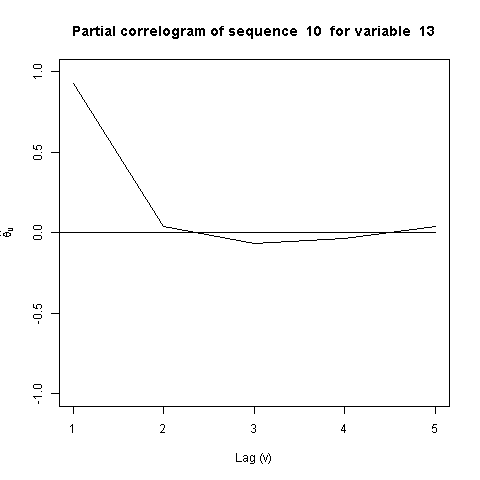
\includegraphics[width=70mm]{figures/CajamarPartialCorrelogram}
    \end{tabular}
     \caption{\label{fig:CajamarCorrelogramsAndPartial} Correlogram and partial correlogram for a variable. A first order Markov assumption seems reasonable to capture dependences over time.}
\end{figure}


Finally, an indicator variable $\delta_{X_t}$ may be included if the variable contains 0 values many times. This is the case for every day payments made by credit card or the historical monthly outstanding amount on the account for instance, whose value can be equal to zero for a large number of days for most customers. For example, Figure \ref{fig:CajamarZeroes} (left) displays the histogram of a variable including all values, and Figure \ref{fig:CajamarZeroes} (right) when the zero values are not considered. Note that the fitted density when the zeroes are discarded are extremely more representative that including zeroes. This result undoubtedly justifies the use of this indicator variable.

\begin{figure}[h]
  \centering
    \begin{tabular}{cc}    
       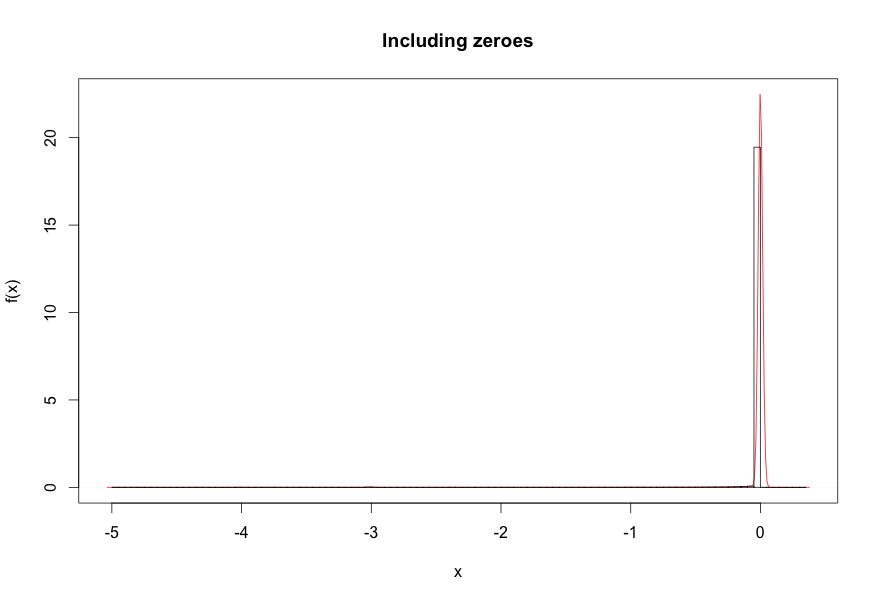
\includegraphics[width=70mm]{figures/with_zeroes}&
       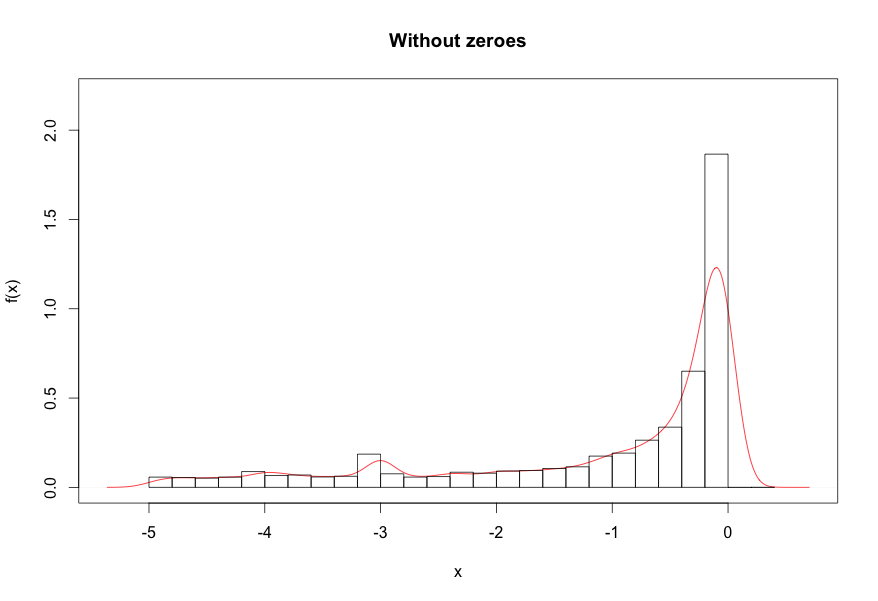
\includegraphics[width=70mm]{figures/without_zeroes}
    \end{tabular}
    \caption{\label{fig:CajamarZeroes}Data histograms and fitted densities for the same variable including zeroes (left) and discarding them (right). In both cases, outliers have been removed for a clearer representation.}
\end{figure}

On the other hand, there exist some variables that, even though some dependences over time would expected, they do not display any type of dynamic behaviour. This is for instance the case for variables whose correllograms in Figure \ref{fig:cajamarCorr} show values very close to zero for all lags. These variables are hence not linked through consecutive time steps in the dynamic model and are represented by $Y_{t+1}$ in Figure \ref{fig:component} together with sociodemographic variables.

\begin{figure}[h]
  \centering
    \begin{tabular}{cc}
    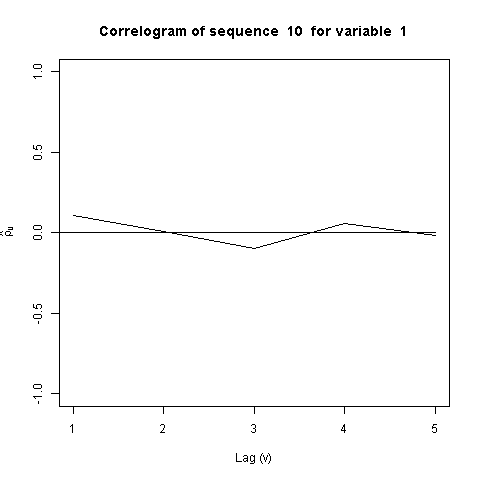
\includegraphics[width=70mm]{figures/CajaMarcrl1}&
     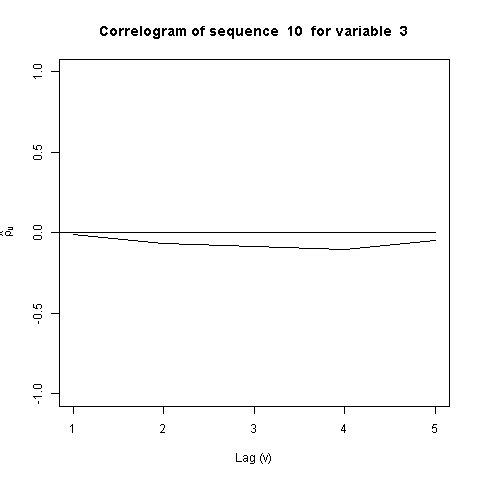
\includegraphics[width=70mm]{figures/CajaMarcrl3}\\
  \end{tabular}
    \caption{\label{fig:cajamarCorr}Correllogram for two variables. No temporal dynamic is shown.}
\end{figure}

In summary, the process of building this dynamic model from the original relational database 
is exactly the same as for the static model.

%%%%%%%%%%%%%%%%%%%%%%%%%%%%%%%%%%%%
\subsubsection{Low risk profile extraction} \label{subsubsec:profileExtraction}
%%%%%%%%%%%%%%%%%%%%%%%%%%%%%%%%%%%%
\subsubsection*{Introduction of the problem}

The marketing department at Cajamar periodically launches marketing campaigns for the recruitment of new products by customers (i.e. a new credit card, an insurance, ...). The success of these campaigns depends greatly on the client group to which the campaign has finally targeted. It is also crucial to reduce as much as possible unnecessary expenses focused on non-potential customers. 

For this purpose, the marketing group proceeds as follows. First, they filter the customers using their own marketing models and also, in collaboration with the risk department, select a subset of predictors considered relevant to be part of the final profile (mainly sociodemographic variables). For example, the age of a client is a relevant predictor when designing campaigns to attract customers for a death insurance. 

After obtaining this first group of customers for the campaign and determining the set of relevant attributes, the model proposed in Section~\ref{SubSection:Predicting} will be used to identify the profiles of the less risky clients using the most probable explanations (MPE) method (\emph{defaulter} variable is evidenced to \emph{No}) . Thus, the target customers previously filtered can be now grouped and ranked using these profiles.


\subsubsection*{Static model}
\label{sec:StaticModel}

As pointed out before, mainly sociodemographic variables will determine the customer profiles used in the campaigns. These variables are mostly static as they do not change frequently over time (e.g. marital status, sex, type of job, ...). However, to enhance the analysis a number of  variables changing over time will be included, although due to complexity reasons we should reduce this number as much as possible to make the profile extraction problem feasible.
The structure for the static model proposed in the profile extraction is the same as for predicting the risk of defaulting (see Fig.~\ref{fig:CajaMarModel0}) but with a considerable reduction in the number of predictors used. 

%\begin{figure}[h]
%\centering
%%\begin{tikzpicture}[->,>=stealth,shorten >=1pt,auto,node distance=2cm,semithick,
%%        azul/.style={fill=cyan,rectangle,draw},
%%        verde/.style={fill=green,ellipse,draw}]
%%        \node[verde] (default) {Default};
%%        \node[azul] (predictors) [below of=default] {Predictors};
%%        \draw (default) to (predictors);
%%\end{tikzpicture}
%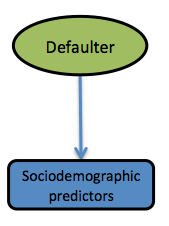
\includegraphics[width=35mm]{figures/CajamarProfileExtractionBN}
%\caption{Static Bayesian network for the profile extraction. The predicting variables can be connected to conform an augmented Bayesian classifier.}
%\label{fig:StaticBNProfile}
%\end{figure}



%---------------------------------------------------------------------------------------------

%
%Note that past information about the variables are not considered for this problem as it was for predicting the probability of defaulting in Section~\ref{SubSection:Predicting}. In this model the latest information about the variables are considered instead.

For the profile extraction, the model not necessarily must have a classifier structure but it can have a general structure instead. However, what is desirable is to avoid using a NB structure for this task. The reason is that once the \emph{defaulter} variable is evidenced to \emph{No}, the predictors become independent and the analysis would be poorer (MPE in this case would correspond to the maximum probability value for each variable individually).



\subsubsection*{Dynamic model}

As mentioned in Section~\ref{sec:StaticModel} the profile extraction problem mainly uses sociodemographic variables but in practice it might happen that variables related to financial activities or paying behaviour are required to be included in this model.  For instance, it could be of interest to include in a profile the tendency of a variable, i.e., the balance of a customer in the last days. For these reasons we should consider the modelling of a dynamic version for the profile extraction. 

The model for the profile extraction is the same as the one depicted in Figure~\ref{fig:component} but, as for the static approach, with a considerable reduction in the number of predictors. 

%\subsubsection*{Model Structure}
%
%From a probabilistic modelling point of view, Caja-Mar faces two different problems [][]: the prediction of the risk of defaulting of a customer in the next two years; and the extraction of profiles of ``desirable'' prospective customers. 
%
%The risk prediction problem has been modelled as supervised dynamic prediction problem.  We are given a data base with a set of variables or predictors (some of them manually built by CajaMar's experts) describing the financial behaviour of the customers and, also, whether the customer is considered as defaulter and non defaulter according to CajaMar standards (i.e. a binary class variable). The dynamic component of the problem needs to be considered because the behaviour of the customers evolves over time (e.g. the account balance is continuously changing from month to another, the level of incomes, etc.)  as well as the labelling as defaulter or non-defaulter customer (e.g. one customer can be creditworthy and, but after some time, be in bankrupt for becoming unemployed). More specifically, the proposed model is expected to answer the following question: which is the probability that this customer will  default in some of his/her loans in two years? And this prediction has to be made only using the customer's behavior in the last 180 days \footnote{This limit is imposed by the Bank of Spain.}.
%
%The graphical structure of the dynamic probabilistic graphical model devised for this problem is given in Figure \ref{Figure:CajaMarModel1}.  The yellow square boxes ``Day -180'', ..., ``Day-1'' represents the temporal evolution of the predictor variables. The model only refers to 180 days because this is the imposed limit of days when making predictions. Similarly, the class variable ``default'' is assumed to evolve over time but with the relevant different that the default class sequence refers to a point in the time \textbf{two years later} than  the point in the time the daily predictor variables. 

\subsubsection{Discussion and future models}

Models presented above are a first attempt to address the tasks involved in Cajamar problem. Thus, this section is mainly devoted to state that some of the proposals might be slightly modified to achieve the requirements presented in~\cite{Fer14b} and to face other unexpected events.

The static model shown in Figure~\ref{fig:CajamarStaticModel} for predicting the probability of default is assumed to have only dependences among variables within each group of variables (white boxes). However, according to expert knowledge, no limitations should be imposed to the model structure among the predicting variables. Figure~\ref{fig:staticDependences} shows the modified structure of the static model when dependences among predicting variables are allowed, meaning that, variables within the dashed blue box could be connected as well. Note that, in this case, complexity grows considerably but, it is worth considering this approach to capture dependences that intuitively are not expected and therefore the analysis will be enriched.

\begin{figure}[htbp]
  \centering
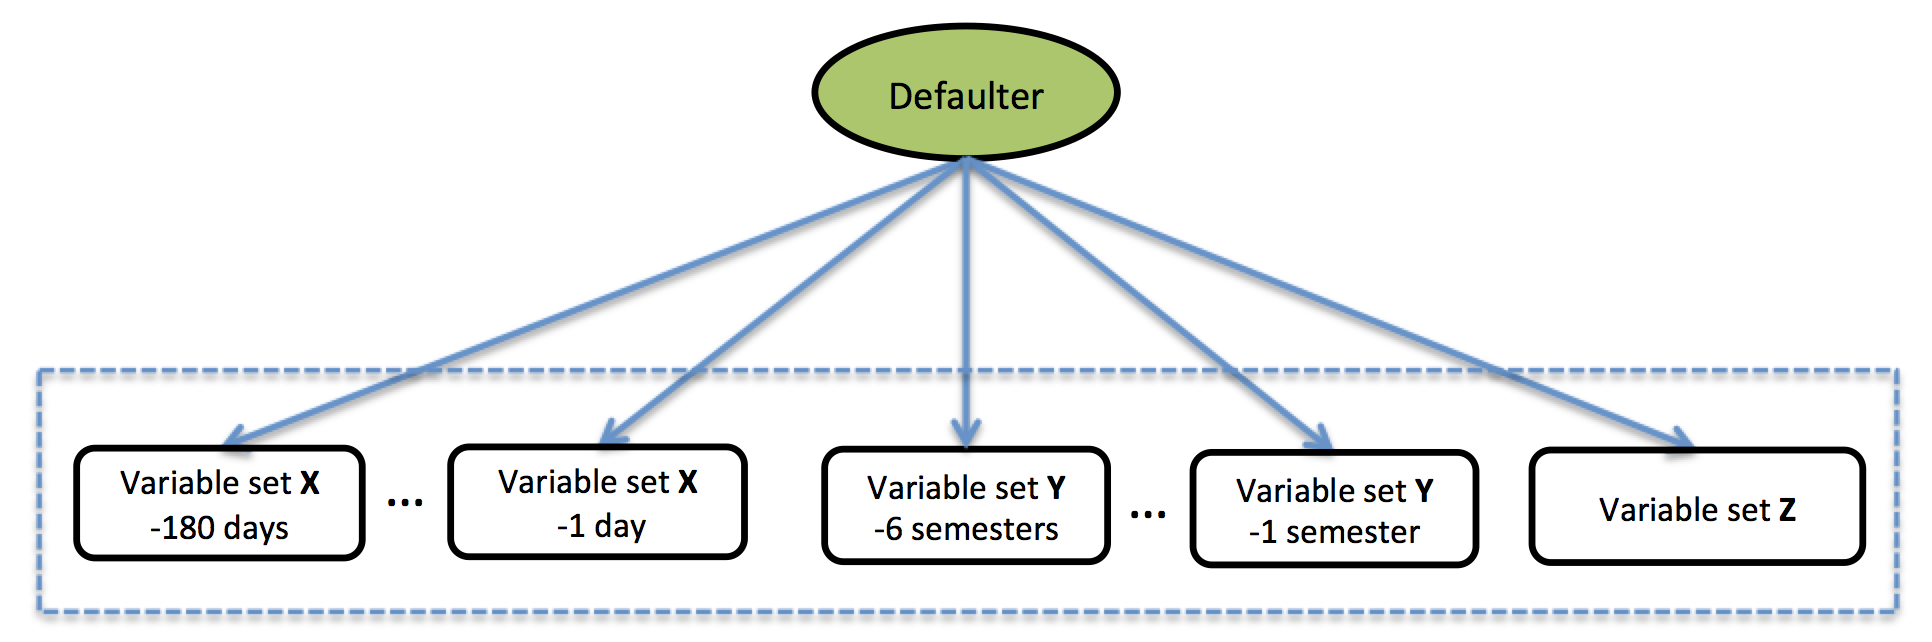
\includegraphics[scale=0.35]{./figures/CajaMarModel3}
\caption{\label{fig:staticDependences}Global structure of the static model allowing dependences among any variable within the dashed blue box. Each white box represents a set of variables for a particular time. The green node on top is the class variable \emph{Defaulter} that represents the probability that a customer will default within the next two years.} 
\end{figure}

%%%%%%%%%%%%%%%%%%%

In general, the model structure in Figure~\ref{fig:staticDependences} can not be modeled by CG distributions (see Section\ref{sec:}). If so, other probability distributions families will be explored. Mainly, they consist in translating the probability distribution into another such that learning and inference become feasible. These approaches include discretization or more complicated families based on Mixture of Truncated Basis Functions~\cite{Lan12}, which can cope with any generic model structure.


%%%%%%%%%%%%%%%%%%

Another issue to be considered is about complexity in the profile extraction task explained in Section~\ref{subsubsec:profileExtraction}. It is well known that abductive inference over BNs and, in particular, the computation of the most probable explanations (MPEs) is an NP-hard problem~\cite{Shi94}. Thus, the model presented in Figure~\ref{fig:staticDependences}, which is valid for the profile extraction as well, could be simplified if necessary
by manually reducing the number of predictors in such a way that computational burden is adapted to the needs. In fact, this process is tightly connected to the expert knowledge provided by the marketing group, and this refinement would not be a problem.

%%%%%%%%%%%%%%%

The model for predicting the risk of default is assumed to be learnt every day. However, if required, this assumption can be relaxed and the learning process could be carried out less frequently. The results hardly will be affected as one-day data have little impact in comparison with the historical data captured in the current model so far. Note that, even if the model is not update, the risk predictions are computed every day using the latest model available so far.



